% !TEX root = seminararbeit.tex

\section{Conclusion}\label{results}

% Die vorliegende Arbeit beschäftigt sich mit der iterativen Entwicklung einer
% Augmented Reality Anwendung für das Android-Betriebssystem. Ziel dabei war es
% eine Anwendung zu entwerfen, die als Vorlage für die Generierung mittels der
% SSIML-Sprachfamilie dient. Dafür wurden ver- schiedene bereits vorhandene
% Frameworks auf ihre Tauglichkeit für diesen Zweck überprüft. Da- nach wurde
% ein High-Level Framework für Android entworfen, mit welchem es möglich ist
% durch minimalem Programmieraufwand eine Augmented Reality Anwendung zu erzeugen.
% Dieses Fra- mework dient als Adapter zu low-level Frameworks und reduziert den
% vom Entwickler benötigten Quellcode auf ein Minimum, wodurch eine
% Codegenerierung mittels domänenspezifischer Spra- chen gut umgesetzt werden
% kann. Leider war es nicht möglich bestimmte Eigenschaften einer Augmented
% Reality Anwendung umzusetzen da sie den Rahmen dieser Arbeit sprengen würde.
% Das Überlagern von 3D-Objekte durch ein reales Objekt, oder ein sich nach der
% Umgebungs- beleuchtung anpassendes Lichtsystem gehören hier zu. Außerdem wäre
% es möglich das Sensor System um Kollisionssensoren oder Annäherungssensoren zu
% erweitern. Abschließend kann fest- gestellt werden, das Hilfe des in dieser
% Arbeit vorgestellte Augmented Reality Framework es mög- lich ist eine
% performante AR-Anwendung ohne große Probleme mittels der SSIML-Sprachfamilie zu
% Erzeugen.

%TODO: motivation wiederholen
% as described in
% probleme mit anderen tools
% mein tool macht das nicht

The presented work explores the planning and the implementation of a \gls{3D} composition tool. The created scene composition tool, \gls{SceGraToo}, enables the user to:

\begin{itemize*}
  \item Upload a \gls{R3D} project,
  \item visualize the scene,
  \item translate, rotate and scale any 3D object,
  \item remove 3D objects,
  \item reorder the the 3D objects in the the tree-view,
  \item add new objects via dragging them over the tree-view and dropping them on any group or transform node,
  \item save the changed scene on the server and
  \item download it again.
\end{itemize*}

And all of that is possible from within the browser.
The downloaded project can be further processed with he R3D framework.
What couldn't be implemented, due to time constraints, is a way to synchronize a scene between browser sessions and allow multiple users to change one scene.

\subsection{Example}

In the following I'll demonstrate an example. Listing \ref{list:cubes} shows an X3D scene with 3 cubes. All 3 cubes lie in the origin of the coordinate system (see Figures \ref{fig:origin} and \ref{fig:origin-tree}).
After moving the cubes via the 3D scene and refining their translations via the tree view (Figure~\ref{fig:stack-tree}) the cubes appear stacked, as can be seen in Figure~\ref{fig:stack}.
In Listing \ref{list:stack} the changes transform nodes can be seen.

\begin{listing}
  \begin{minted}[breaklines,bgcolor=bg]{xml}
<group>
  <transform translation="0 0 0">
    <inline>
      <Shape>
        <Appearance>
          <Material></Material>
        </Appearance>
        <Box></Box>
      </Shape>
    </inline>
    <transform translation="0,0,0">
      <inline>
        <Shape>
          <Appearance>
            <Material></Material>
          </Appearance>
          <Box></Box>
        </Shape>
      </inline>
      <transform translation="0,0,0">
        <inline>
          <Shape>
            <Appearance>
              <Material></Material>
            </Appearance>
            <Box></Box>
          </Shape>
          <Shape>
            <Appearance>
              <Material></Material>
            </Appearance>
            <Box></Box>
          </Shape>
        </inline>
      </transform>
    </transform>
  </transform>
</group>
  \end{minted}
  \caption{A group with 3 nodes with all transform's translation attributes set to \texttt{0,0,0}.}
  \label{list:cubes}
\end{listing}

\begin{listing}
  \begin{minted}[breaklines,bgcolor=bg]{xml}
<group>
  <transform translation="0 0 0">
    <inline>
      <Shape>
        <Appearance>
          <Material></Material>
        </Appearance>
        <Box></Box>
      </Shape>
    </inline>
    <transform translation="0,3,0">
      <inline>
        <Shape>
          <Appearance>
            <Material></Material>
          </Appearance>
          <Box></Box>
        </Shape>
      </inline>
      <transform translation="0,3,0">
        <inline>
          <Shape>
            <Appearance>
              <Material></Material>
            </Appearance>
            <Box></Box>
          </Shape>
          <Shape>
            <Appearance>
              <Material></Material>
            </Appearance>
            <Box></Box>
          </Shape>
        </inline>
      </transform>
    </transform>
  </transform>
</group>
  \end{minted}
  \caption{A group with 3 nodes where two transforms' translation attributes are set to \texttt{0,3,0}, thus stacking the cubes.}
  \label{list:stack}
\end{listing}

\begin{figure}
  \centering
  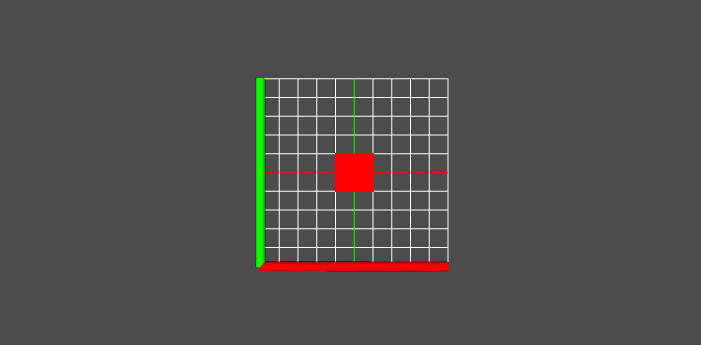
\includegraphics[width=\textwidth]{../assets/origin.png}
  \caption{3 cubes, all centered in the origin of the coordinate system.}
  \label{fig:origin}
\end{figure}
\begin{figure}
  \centering
  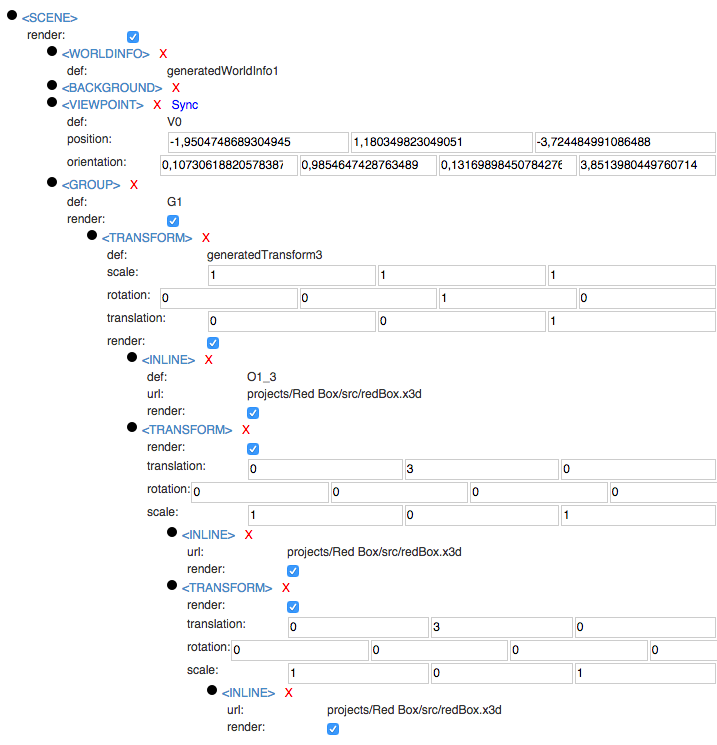
\includegraphics[width=\textwidth]{../assets/origin-tree.png}
  \caption{The tree view corresponding to Figure~\ref{fig:origin}.}
  \label{fig:origin-tree}
\end{figure}
\begin{figure}
  \centering
  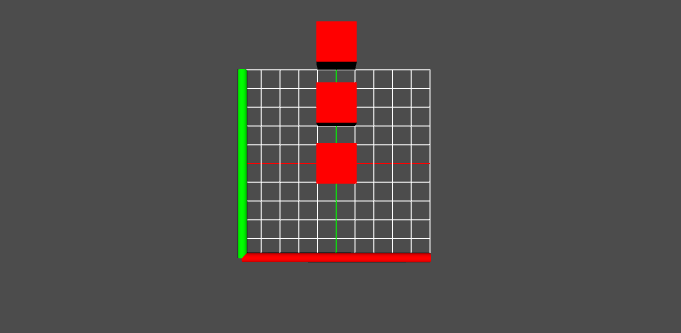
\includegraphics[width=\textwidth]{../assets/stack.png}
  \caption{3 cubes stacked.}
  \label{fig:stack}
\end{figure}
\begin{figure}
  \centering
  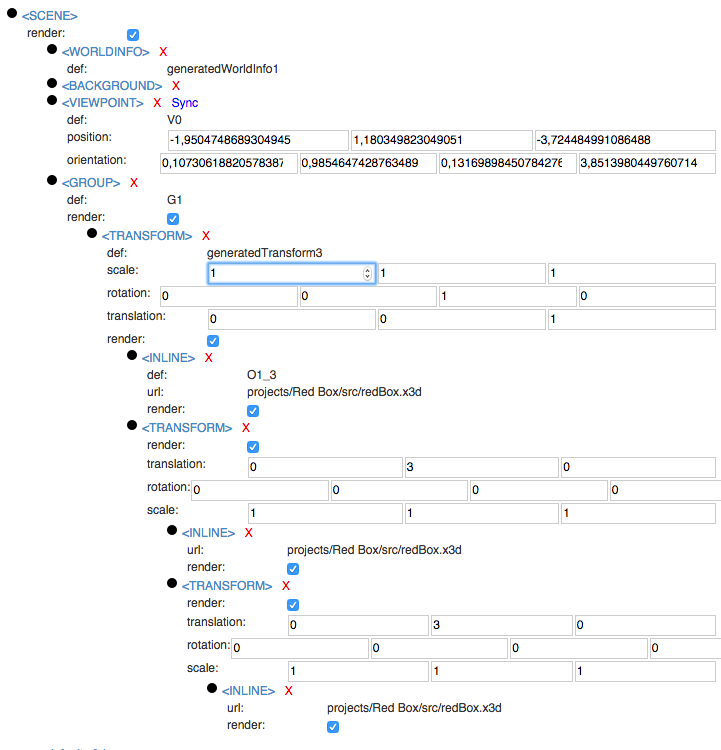
\includegraphics[width=\textwidth]{../assets/stack-tree.png}
  \caption{The tree view corresponding to Figure~\ref{fig:stack}.}
  \label{fig:stack-tree}
\end{figure}
